\documentclass[spec, och, coursework, times]{shiza}
% параметр - тип обучения - одно из значений:
%    spec     - специальность
%    bachelor - бакалавриат (по умолчанию)
%    master   - магистратура
% параметр - форма обучения - одно из значений:
%    och   - очное (по умолчанию)
%    zaoch - заочное
% параметр - тип работы - одно из значений:
%    referat    - реферат
%    coursework - курсовая работа (по умолчанию)
%    diploma    - дипломная работа
%    pract      - отчет по практике
% параметр - включение шрифта
%    times    - включение шрифта Times New Roman (если установлен)
%               по умолчанию выключен

\usepackage{subfigure}
\usepackage{tikz,pgfplots}
\pgfplotsset{compat=1.5}
\usepackage{float}

%\usepackage{titlesec}
\setcounter{secnumdepth}{4}
%\titleformat{\paragraph}
%{\normalfont\normalsize}{\theparagraph}{1em}{}
%\titlespacing*{\paragraph}
%{35.5pt}{3.25ex plus 1ex minus .2ex}{1.5ex plus .2ex}

\titleformat{\paragraph}[block]
{\hspace{1.25cm}\normalfont}
{\theparagraph}{1ex}{}
\titlespacing{\paragraph}
{0cm}{2ex plus 1ex minus .2ex}{.4ex plus.2ex}

% -----------------------------------------------------------------------------%


\usepackage[T2A]{fontenc}
\usepackage[utf8]{inputenc}
\usepackage{graphicx}
\graphicspath{ {./images/} }
\usepackage{tempora}

\usepackage[sort,compress]{cite}
\usepackage{amsmath}
\usepackage{amssymb}
\usepackage{amsthm}
\usepackage{fancyvrb}
\usepackage{listings}
\usepackage{listingsutf8}
\usepackage{longtable}
\usepackage{array}

\usepackage[english,russian]{babel}

%\usepackage[colorlinks=true]{hyperref}
\usepackage{url}


\newcommand{\eqdef}{\stackrel {\rm def}{=}}

\renewcommand\theFancyVerbLine{\small\arabic{FancyVerbLine}}

\newtheorem{lem}{Лемма}

\begin{document}

% Кафедра (в родительном падеже)
\chair{теоретических основ компьютерной безопасности и криптографии}

% Тема работы
\title{отчет}

% Курс
\course{четвертый}

% Группа
\group{431}

% Факультет (в родительном падеже) (по умолчанию "факультета КНиИТ")
\department{факультета компьютерных наук и информационных технологий}

% Специальность/направление код - наименование
%\napravlenie{09.03.04 "--- Программная инженерия}
%\napravlenie{010500 "--- МОАИС}
%\napravlenie{230100 "--- Информатика и вычислительная техника}
%\napravlenie{231000 "--- Программная инженерия}
\napravlenie{090301 "--- Компьютерная безопасность}

% Для студентки. Для работы студента следующая команда не нужна.
% \studenttitle{Студентки}

% Фамилия, имя, отчество в родительном падеже
\author{Иванова Ксения Владиславовна}

% Заведующий кафедрой
\chtitle{д.~ф.-м.~н.,~доцент} % степень, звание
\chname{М.~Б.~Абросимов}

%Научный руководитель (для реферата преподаватель проверяющий работу)
\satitle{доцент} %должность, степень, звание
\saname{А.~А.~Лобов}

% Руководитель практики от организации (только для практики,
% для остальных типов работ не используется)
% \patitle{к.ф.-м.н.}
% \paname{С.~В.~Миронов}

% Семестр (только для практики, для остальных
% типов работ не используется)
\term{восьмой}

% Наименование практики (только для практики, для остальных
% типов работ не используется)
% \practtype{Ознакомительная}

% Продолжительность практики (количество недель) (только для практики,
% для остальных типов работ не используется)
% \duration{2}

% Даты начала и окончания практики (только для практики, для остальных
% типов работ не используется)
% \practStart{22 июня 2020}
% \practFinish{05 июля 2020}

% Год выполнения отчета
\date{2024}

\maketitle

% Включение нумерации рисунков, формул и таблиц по разделам
% (по умолчанию - нумерация сквозная)
% (допускается оба вида нумерации)
% \secNumbering

%------------------------------------------------------------------------------%

\tableofcontents
\intro
В последнее время компании все чаще предпочитают легкие, быстырые и универсальные 
web-приложения для своих услуг, взмен тяжеловесным дестктопным. А из этого 
вытекает появление большого количества фремворков и библиотек для разработки и 
поддержки web-приложений, которые позволяют реализовать все, что необходимо для 
функционирования современного web-приложения.
Поэтому одной из сложностей является выбор подходящего для целей приложения фреймворка, 
а для правильного выбора нужно понимать достоинства и недостатки каждого. В этой работе я 
рассмотрю популярные среди разработчиков фреймворки с точки зрения безопасности, 
расстмотрю их функционал и оценю его работу.

\section{Web-приложение}
\subsection{Структура и работа}
Web-приложение — это клиент-серверное приложение, в котором осуществляется взаимодействие клиента с сервером, за 
счет браузера, а сервером является веб-сервер, который принимает HTTP-запросы от клиента (браузера), и в свою очередь 
выдает HTTP-ответы вместе с HTML-страницей, изображением или какими-нибудь другими данными. Клиенты могут получить доступ
к веб-серверу по URL адресу необходимой им страницы.

Для веб-приложений на стороне сервера можно применять различные технологии и любые языки программирования. 
Для клиента-браузера же не важно на какой ОС оно работает, в этом заключается один из главных плюсов --
кроссплатформенность (Рис.1).
\begin{figure}[H]
  \centering
  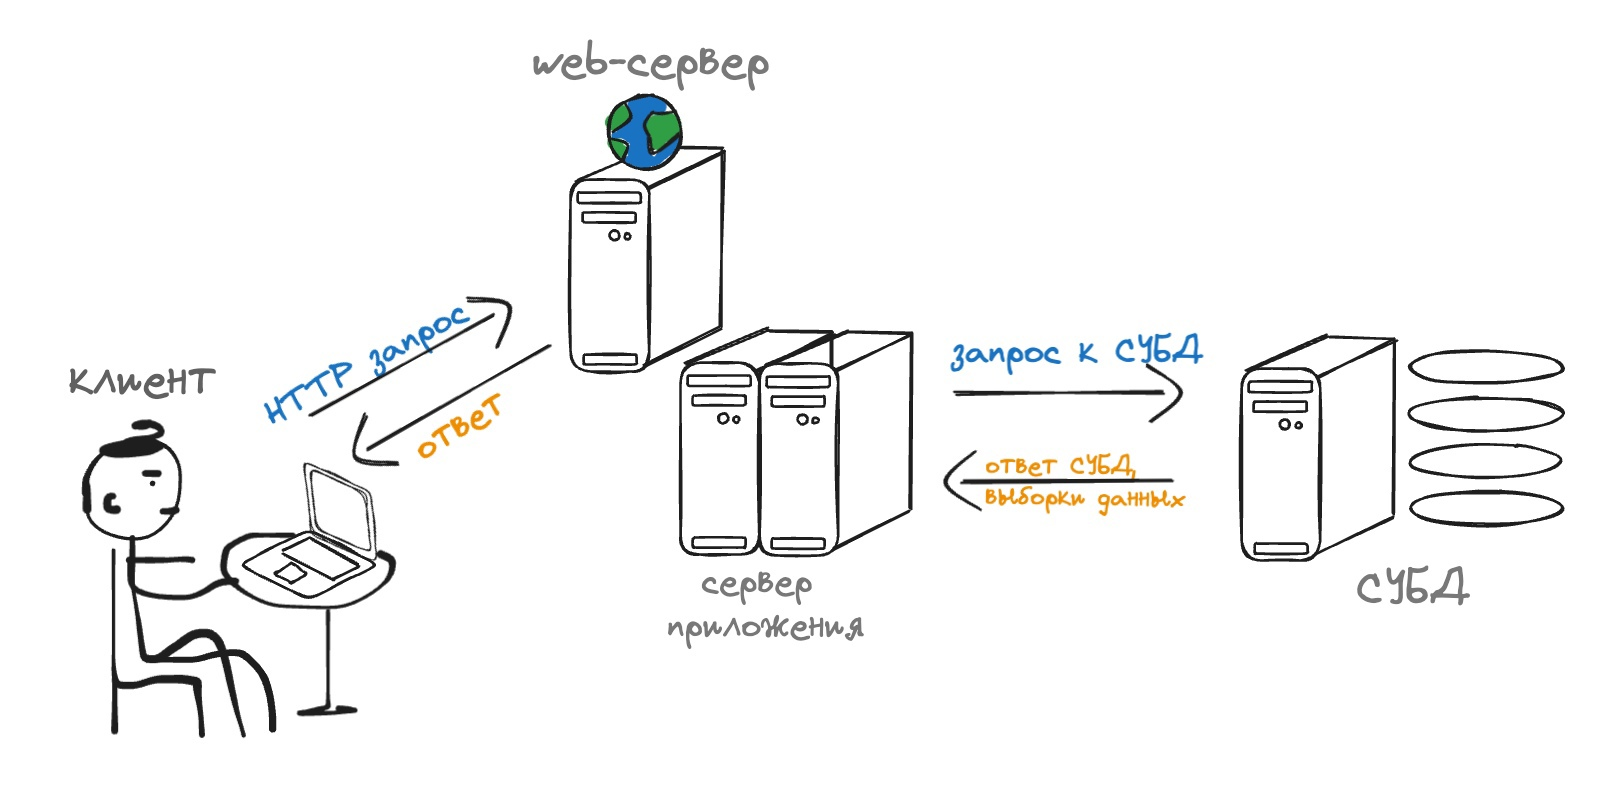
\includegraphics[width=1\textwidth]{pict/1}
  \caption{принцип обработки запросов приложением}
  \label{fig:1}
\end{figure}

Существует четыре общих уровня веб-приложений:
\begin{description}
\item[--]Представления (PL) имеет компоненты пользовательского интерфейса, которые показывают данные для пользователей, также
компоненты пользовательского процесса, которые задают взаимодействие с пользователем. PL предоставляет всю необходимую 
информацию клиентской стороне. Основная цель уровня представления - получить входные данные, обработать запросы пользователей,
отправить их в службу данных и показать результаты.

\item[--]Слой бизнес-логики BLL несет ответственность за надлежащий обмен данными между уровнем представления PL и уровнем обмена данными DAL, определяет логику бизнес-операций и правил. 

\item[--]Службы данных DSL передает данные, обработанные уровнем бизнес-логики, на уровень представления. Этот 
уровень гарантирует безопасность данных, изолируя бизнес-логику со стороны клиента.

\item[--]Доступа к данным DAL предлагает упрощенный доступ к данным, хранящимся в постоянных хранилищах (например XML). 
Уровень доступа к данным также управляет операциями CRUD - создание (C), чтение (R), обновление (U), удаление (D).

\end{description}
\begin{figure}[H]
  \centering
  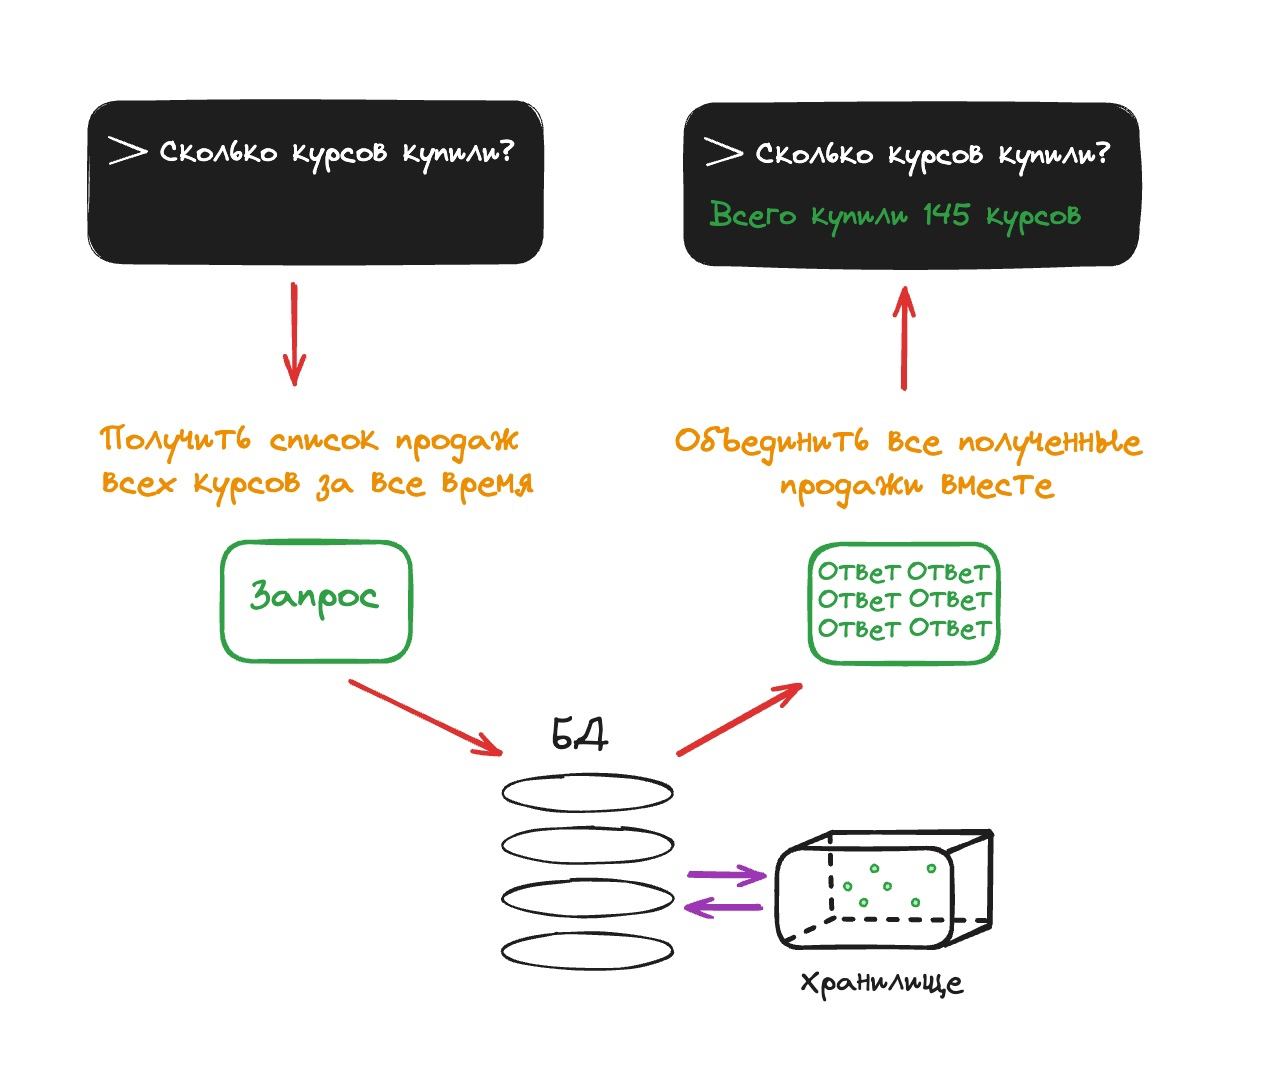
\includegraphics[width=1\textwidth]{pict/2}
  \caption{принцип взаимодействия уровней приложения}
  \label{fig:2}
\end{figure}

Чтобы приложение корректно и безопасно функционировало, необходимо, чтобы на каждом уровне
была обеспечена безопасность передаваемых данных и минимизирована возможность использования особенностей каждого уровня,
в качестве канала получения информации.


\newpage
\subsection{Уязвимости}
При работе с фреймворком разработчик используя функционал чаще всего
ограничивается знанием смысла работы какой-либо функции и ее параметров, не заглядывая внутрь 
нее, не зная всех деталей ее работы. Это большой плюс для разработчика, потому что с помощью
данной «абстракции», он может сконцентрироваться на решение своей задачи, не углубляясь
в ненужные подробности.

Большинство разработчиков не думает о безопасности работы приложения и данных, которыми 
оно оперирует, и тем более не считают это основной задачей, поэтому, если рассматривать
такое качество фреймворка как безопасность, то тем он будет лучше, чем больше будет 
предусматривать и закрывать возможные дыры в безопасности -- уязвимости.

На момент 2024 года такая организация как OWASP (Открытый проект обеспечения безопасности web-приложений) выделила следующие 
популярные уязвимости:
\begin{description}
  \item[--] нарушение контроля доступа;
  \item[--] недочёты криптографии;
  \item[--] инъекции;
  \item[--] небезопасный дизайн;
  \item[--] небезопасная конфигурация;
  \item[--] использование уязвимых или устаревших компонентов;
  \item[--] ошибки идентификации и аутентификации;
\end{description}

\textbf{Нарушение контроля целостности}

Это набор уязвимостей, при которых система плохо контролирует уровни доступа к информации или к своей функциональности.
Из-за этого злоумышленники могут пользоваться функциями, к которым не должны иметь доступа.
Если  веб-приложение, где каждая учётная запись имеет разные права доступа слабо защищено, злоумышленник
может модифицировать запросы или параметры URL, чтобы получить доступ к данным, на которые у него нет права.

\textbf{Недочеты криптографии}

Это уязвимости, связанные с неправильной настройкой и использованием криптографических методов 
для защиты данных. Это может быть недостаточная длина ключей, ненадёжные условия их хранения, использование устаревших 
алгоритмов и другие ошибки в криптографической реализации.

\textbf{Инъекции}

Данный вид уязвимостей -- пользовательский ввод с вредоносным кодом. Инъекции позволяют злоумышленникам внедрять свой вредоносный код 
на сервер и выполнять его. Результат -- потеря данных, кража данных или повреждение системы.

\textbf{Небезопасный дизайн}

Широкая категория уязвимостей, впервые появившаяся в последней версии OWASP Top Ten. Уязвимости этой категории возникают 
потому, что сама логика работы приложения может позволять использовать существующие функции в качестве уязвимостей.

\textbf{Небезопасная конфигурация} 

Это случаи, когда настройки приложения, сервера, базы данных или других компонентов системы 
не являются безопасными. К этому можно отнести ненадёжные или отсутствующие настройки аутентификации, 
авторизации и доступа, например отсутствие защиты от перебора пароля.

\textbf{Использование уязвимых компонентов}

К этому типу уязвимостей относят случаи, когда веб-приложение использует сторонние фреймворки, библиотеки, плагины или 
другие компоненты, которые имеют выявленные дефекты безопасности. У злоумышленников даже есть автоматизированные инструменты,
которые помогают находить неправильно сконфигурированные системы


\textbf{Ошибки идентификации и аутентификации}

Слабые пароли, недостаточная проверка подлинности, неэффективные системы учёта сеансов, все ошибки, которые могут возникнуть
из-за недостаточно безопасной реализации идентификации и аутентификации пользователя в системе.
   
\vspace{2mm}
Можно ли предотвратить реализацию большей части этих уязвимостей, если при разработке использовать определенные фреймворки, а может 
вообще что-то может быть обработано на уровне языка. В последующей своей работе, я рассмотрю самые популярные фреймворки для разработки
web-приложений и попробую проанализировать, какие базовые критерии безопасности они предусматривают. 

\section{Фреймворки для создания Web}
Фреймворк -- это динамически пополняемая библиотека языка программирования, в 
которой собраны его базовые модули. Фреймворки создаются для упрощения процессов разработки приложений, сайтов, сервисов.
Чтобы не писать модуль в приложении с нуля, гораздо проще обратиться к готовым шаблонам фреймворков, которые и формируют 
рабочую среду разработчика.

Архитектура почти всех фреймворков основана на декомпозиции нескольких отдельных слоев (приложения, модули и т. д.) проекта.
Это означает, что можно расширять функциональность приложения исходя из потребностей и использовать измененную версию вместе 
с кодом фреймворка или задействовать сторонние приложения. Такая гибкость является одним из одним из ключевых преимуществ 
использования фреймворков.

Рассмотрим в общем несколько популярных фреймворков и их особенности.

\subsection{ASP.NET (.NET)}
 
Учитывая популярность в свое время технологий .NET, стоит поговорить про такой фреймворк, как ASP.NET -- это набор технологий 
в составе .NET Framework, которые позволяют создавать
web-приложения и сервисы на основе Microsoft.NET с использованием любых поддерживаемых ей языков. В отличие от 
web-страниц, которые представляют собой сочетание статического HTML
и сценариев, платформа использует скомпилированные страницы, которые управляются событиями. Но в отличие от десктопных приложений, эти 
скомпилированные страницы создают информацию, отправляемую клиентам с использованием языков
разметки наподобие HTML и XML. Это позволяет разработчикам создавать приложения, защищая
при этом интерфейс пользователя под управлением разных операционных систем.

Основная концепция безопасности, которая есть в .NET -- прежде всего это ролевая модель безопасности. Она подразумевает 
два основных режима работы. Первый это создание пользователей и ролей, которые не 
зависят от ролей ОС Windows. Такая модель удобна, когда все разграничение прав внутри приложения ведется именно с помощью
ролей. Все это никоим образом не связано с учетными записями в ОС. Например, это доступность
каких-либо компонентов веб приложения в зависимости от заданной роли пользователя.

Второй режим -- жесткая привязка ролей в приложении к учетным записям в Windows. Обычно подобную модель безопасности 
можно встретить в веб-приложениях, работающих во внутренней ё 2среде и тесно связанных с инфраструктурой Active Directory.

Аутентификация в ASP.NET приложениях обычно реализуется или с помощью аутентификации Windows или с помощью форм. Первый
вариант построен на использовании штатных средств операционной системы . В каждом случае пользователь предъявляет некий
аналог “удостоверения” – в первом случае это SID (Security Identifier), а во втором случае формируется так называемый билет,
который затем сохраняется в cookie. 

Для работы с базой данных используется объектно-ориентированная технология доступа к данным -- Entity Framework (EF), которая 
является object-relational mapping (ORM) решением для .NET Framework от Microsoft. Изначально с самой первой версии Entity Framework поддерживал подход 
Database First, который позволял по готовой базе данных сгенерировать edmx модель данных файла. Затем эта модель использовалась для 
подключения к базе данных. Позже был добавлен подход Model First. Он позволял создать вручную с помощью визуального 
редактора модель, и по ней создать базу данных. Предпочтительным подходом стал Code First, в котором сначала пишется код 
модели, а затем по нему генерируется база данных.

\textbf{Положительные стороны:}
\begin{itemize}
  \item[-] Возможность разработки крупных проектов со сложной архитектурой;
  \item[-] Совместимость с несколькими операционными системами; 
  \item[-] Разработка на разных языках;
\end{itemize}


\textbf{Отрицательные стороны:}
\begin{itemize}
  \item[-] Проблемы с одновременным доступом большого числа пользователей;
  \item[-] Используется компиляция, при незначительных нагрузках сервисы работают медленнее;  
  \item[-] При разработке приложений используются лицензированные инструменты, что приводит к удорожанию продукта.
\end{itemize}


\subsection{Laravel (Php)}
На конец 2023 года, по статистике GitHub, Php занимает 7 место по популярности среди всех существующих языков разработки[6].
Так или иначе этот язык присутствует в 79,2 \% от общего числа всех вебсайтов в интернете, не удивительно, ведь он стоял у истоков интернета.
Один из популярнейших фреймворков Php -- Laravel считается довольно простым для входа среди всех Php-фреймворков, т.к делает процесс разработки веб-сайтов проще и быстрее из-за
простой обработки кода, и множества встроенных модулей. Что важно фреймворк содержит пакет безопасности, который позволяет повысить защищенность приложения.

Внутри фреймворка Laravel есть свой ORM -- Eloquent. В библиотеке ORM помимо стандартных CRUD-операций можно выделить наличие методов доступа,
мутаторов, безопасное удаление, направления областей запросов, построения отношений, построение взаимодействия на основе событий. 
Eloquent организует работу с базой через представление таблиц в виде <<моделей>>, через которы и осуществляется доступ и манипуляции с данныими.

\textbf{Положительные стороны:}
\begin{itemize}
  \item[-] простая интеграция платежных шлюзов;
  \item[-] встроенные пакеты шифрования, основанные на OpenSSL в системе алгоритмов AES-256 и AES-128; 
  \item[-] наличие встроенных шаблонизаторов Blad;
  \item[-] частая обновляемость и поддержка.
\end{itemize}

\textbf{Отрицательные стороны:}
\begin{itemize}
  \item[-] большой объем файлов и зависимостей, что может навредить производительности;
  \item[-] несовместимость обновлений фреймворка, что может привести к конфликтам внутри проекта.
\end{itemize}
   
    
Некоторые пункты, которые реализует фреймворк в плане безопасности.

\textbf{Токены CSRF}

Laravel автоматически генерирует «токен» CSRF для каждой активной пользовательской сессии, управляемой приложением.
Он используется для проверки, что аутентифицированный пользователь не является злоумышленником.

\textbf{Защита от XSS}

Laravel автоматически экранирует выводимые данные, чтобы предотвратить XSS-атаки. Чтобы безопасно выводить данные, используется Blade-синтаксис (шаблонизатор).

\textbf{Защита от SQL}

Существует несколько различных способов защиты от SQL-инъекций.


\subsection{Django (Python)}
Высокоуровневый фреймворк, который является не только быстрым решением в веб-разработке, включающим все необходимое для 
качественного кода и прозрачного написания, но и также удобным для разработчиков.
В Django реализован принцип DRY — Don't Repeat Yourself (не повторяйся). То есть при использовании Django не нужно 
несколько раз переписывать один и тот же код. Фреймворк позволяет создавать сайт из компонентов. Благодаря этому сокращается 
время создания сайтов.

Фреймворк справляется с большим количеством задач и повышенными нагрузками, также подходит для создания алгоритмических 
генераторов, платформ для электронных рассылок, систем верификации, платформ для анализа данных и сложных вычислений, машинного обучения.
У фреймворка есть своя ORM, которая автоматически передает данные из БД в объекты,
которые используются в коде приложения, включает механизмы предотвращения распространенных атак вроде SQL-инъекций 
и подделки межсайтовых запросов.

\textbf{Положительные стороны:}
\begin{itemize}
 \item[-] масса различных библиотек;
 \item[-] подробная документация и очень развитое сообщество;
 \item[-] возможность масштабирования по мере необходимости.
\end{itemize}

\textbf{Отрицательные стороны:}
\begin{itemize}
 \item[-] нет поддержки WebSockets;
 \item[-] Django ORM сегодня значительно уступает последней SQLAlchemy.
\end{itemize}

Некоторые пункты, которые реализует фреймворк в плане безопасности.

\textbf{Внедрение SQL}

Это предотвращается благодаря API QuerySet, который не делает никаких действий с базой,
пока набор запросов к ней не будет обработан. 

\textbf{Параметризация}

Он параметризует запросы и абстрагируется от разработчиков. Готовые шаблоны сами по себе защищают от атак с использованием межсайтовых сценариев.


\textbf{Защита паролей}

Используется функция защиты паролей PBKDF2.о функция получения ключа, разработанная
RSA Laboratories, используемая для получения стойких ключей на основе хеша. Она работает путем применения псевдослучайной хеш-функции к паролю
и повторение этого процесса большое количество раз.

\textbf{Защита от CSRF}

По умолчанию промежуточное ПО CSRF активировано в MIDDLEWARE настройках (CSRF защита теперь является частью ядра Django), а также можно использовать 
его методы для определенных представлений.

% \subsection{Actix (Rust)}
% \subsection{Revel (Gо)}

\newpage

\section{Практическая часть}

\subsection{Критерии оценки безопасности фреймворков}
Может получится много ситуаций, когда приложение, его компоненты или язык на котором это все написано,
ведут себя непредсказуемо, это может быть связано с неправильной обработкой символов, отсутствием проверки каких-либо данных, 
передачи информации без надлежащей защиты ее или самого сеанса, поэтому попробую сформулировать некоторые критерии для фремворка web-приложения,
которые помогут оценить на сколько в плане безопасности продуман функционал.

% \textbf{Правильная обработка символов Юникода}
% Если такие символы, как пробелы и пунктуация, передаются в HTTP, может произойти ситуация, в которой на принимающей стороне
% символы могут быть истолкованы неверно. HTML-кодирование преобразует символы,
% которые не разрешены в HTML, в более менее подходящие аналоги, которые HTML поддерживает.


% \textbf{Влияние нулевых байтов}
% Возможна крайне неожиданная обработка нулевого байта. Строки, содержащие такой байт, могут обработаться только частично, до той позиции, в которой находится этот байт.

% \textbf{Поддержка параметризованных запросов к БД}
% Параметризированные запросы помогают избежать выдачи SQL-м данных из база, с помощью которого можно не допустить прямого ввода данных пользователем в запрос, а вместо этього
% использовать уже готовые шаблоны.

% \textbf{Защита от XSS}
% выполнения требуемой кодировки на основе местоположения вывода, чтобы предотвратить уязвимости межсайтового скриптинга? 
% (если нет, то шаблонизаторы, опасные теги, фильтрация тегов в подстановке html)

% \textbf{Безопасность реализации сеанса, доступ к ОРМ}
% Как происходит генерация токенов, возможно длительность сеанса. Сессия связи с бд, 
% защищенность.

% \textbf{Безопасность механизма аутентификации}

% Блок работы с бд:

% \textbf{Нормализация пути}

% \textbf{Безопасные варианты хранения}

% \textbf{Защита от инъекций строки для записи безопасных журналов}

% \textbf{Функция применения белого списка на входах}



\newpage
\subsection{ASP.NET (.NET)}


\newpage
\subsection{Laravel (Php)}


\newpage
\subsection{Django (Python)}
% \subsection{Actix (Rust)}
% \subsection{Revel (Gо)}


\newpage
\subsection{Сравнение защищенности}

\small
\centering
\begin{flushleft}
\begin{tabular}[t]{|p{9cm}|l|l|l|} \hline 
Фреймворки   Критерии& ASP.NET & Laravel & Django\\[3mm]\hline
Правильная обработка символов Юникода & + & + & + \\[2mm]\hline
Влияние нулевых байтов & + & +& + \\[2mm]\hline
Поддержка параметризованных запросов SQL & + & + & +\\[2mm]\hline
Наличие способа разделения данных и HTML & + & + & +\\[2mm]\hline
Безопасность реализации сеанса, безопасный доступ к ОРМ & + & + & +\\[2mm]\hline
Безопасность механизма аутентификации & + & + & +\\[2mm]\hline
\end{tabular}
\end{flushleft}

\centering
\begin{flushleft}
\begin{tabular}[t]{|p{9cm}|l|l|l|} \hline
Фреймворки  Критерии& ASP.NET & Laravel & Django\\[3mm]\hline
Нормализация пути & + & + & + \\[2mm]\hline
Безопасные варианты хранения & + & +& + \\[2mm]\hline
Защита от инъекций строки для записи безопасных журналовSQL & + & + & +\\[2mm]\hline
Функция применения белого списка на входах \newline шаблонизаторы, опасные теги & + & + & +\\[2mm]\hline
\end{tabular}
\end{flushleft}


\newpage
\conclusion

спать надо
% \begin{figure}[H]
%     \centering
%     \includegraphics[width=1\textwidth]{4.1}
%     \caption{Настройка фильтра №1 на операции RegSetValue и RegCreateKey, а также фильтра №2 на операции WriteFile и CreateFile}
%     \label{fig:8}
% \end{figure}

\begin{thebibliography}{99}
  \bibitem{Andriyanov} Андриянов В. В., Зефиров С. Л., ``ОБЕСПЕЧЕНИЕ ИНФОРМАЦИОННОЙ БЕЗОПАСНОСТИ БИЗНЕСА'', г. Москва, Издательство Альпина Паблишер, 2011 г., Яз. Рус.
  \bibitem{Gruzdev} Груздев С., Сабанов А., ``Вопросы идентификации и аутентификации при разработке мультиаппликационных карт'', [Электронный ресурс] / URL:\\ https://www.aladdin-rd.ru/company/pressroom/articles/voprosy\_identifikacii\_\\i\_autentifikacii\_pri\_razrabotke\_multiapplikacionnyh\_kart, дата обращения 01.07.2020, Яз. Рус.
  \bibitem{Korzhov} Коржов В., ``Пароль на минуту'', [Электронный ресурс] / URL: \\https://www.osp.ru/cw/2005/01/84855/, дата обращения 01.07.2020, Яз. Рус.
  \bibitem{Sabanov} Сабанов А., ``О технологиях идентификации и аутентификации'', [Электронный ресурс] / URL: https://www.aladdin-rd.ru/company/pressroom/articles/o\_\\tehnologiah\_identifikacii\_i\_autentifikacii, дата обращения 01.07.2020, Яз. Рус.
  \bibitem{Fisenko} Фисенко Л., ``Новое лицо киберпреступности'', [Электронный ресурс] / URL:\\https://www.itweek.ru/infrastructure/article/detail.php?ID=71779, дата обращения 01.07.2020, Яз. Рус.
  \bibitem{Fiso} PHP Framework List: An Ultimate Guide to 102 PHP Frameworks for Web Developers [Электронный ресурс]. URL: https://www.temok.com/blog/php-framework-list/ (дата обращения: 25.12.2022).
\end{thebibliography}

\end{document}